\section{{\prg singleion}\index{singleion} - a Crystal Field Program
for Calculating Energy Levels, Transition Matrix Elements etc.}\label{cfield}

\subsection{Doing Single Ion Calculations}
\label{cfieldsep}

The crystal field is the electrostatic field, which is produced by the
charges of the crystal environment of a rare earth atom. It acts on the
4f electrons of the rare earth and causes magnetic anisotropy. Fig.~\ref{chrgpla} and
\ref{chrgplb} show the effect of this field on the charge distribution.
Such plots can be made by using the programs {\prg pointc\index{pointc}} to calculate
the crystal field parameters and
 {\prg display\_density\index{display\_density}} to plot the charge density, see section \ref{addprog}.

\begin{figure}[hb]
\includegraphics[angle=0,width=0.7\columnwidth]{figsrc/crystalfieldplot.eps}
\caption{\label{chrgpla}
The crystal field model: the figure shows the influence of two positive 
charges on the charge density of 4f-electrons. The
charge density is distorted by the electric field from the neighbouring atoms.
Furthermore, this distortion leads to an anisotropy of the magnetic properties
of the 4f shell. The resulting 
easy direction of the magnetic moment is shown by arrows for the different tri positive
rare earth ions.} 
\end{figure}

\begin{figure}[ht]
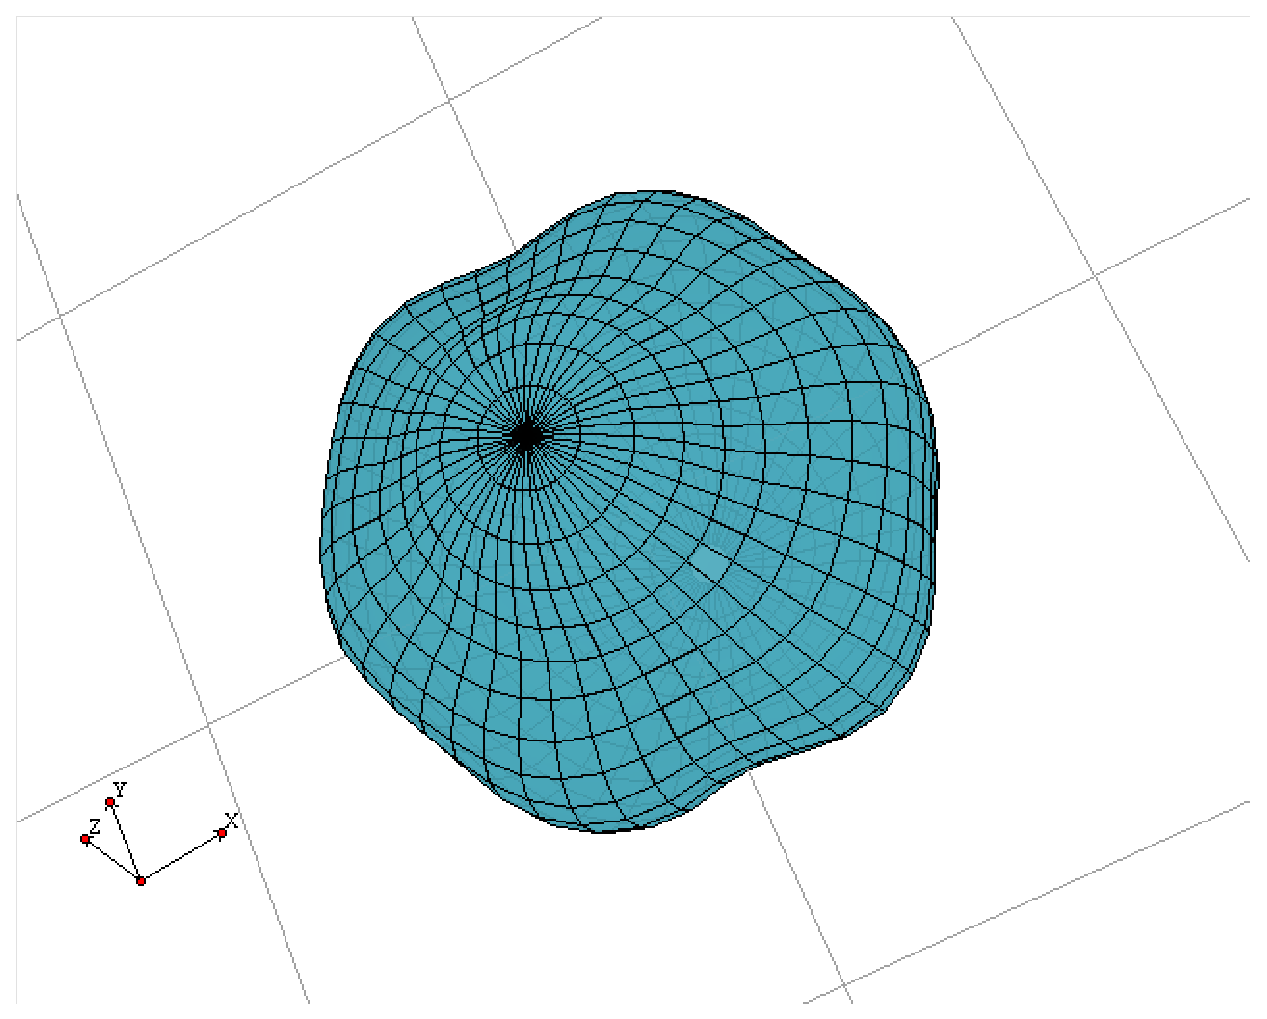
\includegraphics[angle=0,width=0.7\columnwidth]{figsrc/chrgpla.eps}
\caption{\label{chrgplb}
Calculated charge density of 4f-electrons in an orthorhombic crystal field. In
this example the charge density of a Nd$^{3+}$ ion at a temperature of 10~K was 
calculated by taking the crystal
field parameters determined by neutron spectroscopy and 
magnetic measurements in NdCu$_2$~\cite{gratz91-9297}.
[plot created by program {\prg display\_density\index{display\_density}}]}
\end{figure}

We will describe now, how the crystal field influence can be quantitatively evaluated
and how {\prg so1ion}\index{so1ion}  can help to do this.
Within the $|JLSm_J \rangle$ ground state multiplet of the 4f electron wave function 
the crystal field can be described by the following Hamiltonian:

\begin{equation}
\label{cfham}
 {\mathcal H}= \sum_{n,lm} B_{lm} O_{lm}({\mbf J}^n) 
	     - \sum_{n} g_{Jn} \mu_B {\mbf J}^n {\mbf H} 
\end{equation}

The first term in equ.~\ref{cfham} describes the crystal field, the second the
effect of a magnetic field (Zeeman term). The strength of the crystal field is given by the
crystal field parameters $B_l^m$. In the case of isolating materials these
parameters can be obtained by the point charge model (point charges on the 
neighbouring atoms, for details on these calculations see~\cite{hutchings64-227},
in the {\prg McPhase} suite use programs {\prg makenn} and {\prg pointc} to evaluate
the pointcharge model for a given crystal structure, see section~\ref{addprog}).
For metals the conduction electrons screen the point charges and the determination
of the crystal field is usually only possible by fits to experimental data. 
The program package {\prg McPhase} may be used to solve such crystal field problems.

A simpler way of dealing with crystal field anisotropy is to write
instead of the first term in equ.~\ref{cfham}

\begin{equation}
  \sum_s D_x^2 (J_x^s)^2 + D_y^2 (J_y^s)^2 +D_z^2 (J_z^s)^2 
\end{equation}

In order to implement a full diagonalisation of the single ion crystal field Hamiltonian
the module {\prg so1ion}\index{so1ion}({\prg cfield\index{cfield}}, written by P. Fabi n\'e Hoffmann) has %%@
been included into the program package. It  can be used  to 
calculate crystal field problems for rare earth ions. There is a program 
{\prg so1ion}\index{so1ion}, which is self explaining, provided 
the user has a basic knowledge of crystal field 
theory (see e.g. the famous article by Hutchings~\cite{hutchings64-227}).
Here we describe how to use the program {\prg singleion} to do crystal field calculation
for rare earth ions. 

\subsection{Example - how to evaluate the crystal field of NdCu$_2$ using
 {\prg singleion}\index{singleion}}\label{cfieldexample}


A simple input file is made up in the following:

\begin{itemize}
\item The first line in the input file sets the type of single ion module, for rare earth in spin-orbit
    coupling we use {\prg so1ion}\index{so1ion}.
\item Comment lines start with \#. 
\item The type of ion has to be given plus
several lines containing the crystal field parameters. 
\end{itemize}

It follows an example, we take the values
for NdCu$_2$ from literature~\cite{gratz91-9297}. Note that
if the crystal field parameters are not known, there are different
possibilities to obtain values, such as ab initio calculation,
point charge calculations (use module {\prg pointc\index{pointc}}) and fitting
to experimental data (see section~\ref{simannfit}).

\begin{verbatim}
#!MODULE=so1ion
#<!--mcphas.cf-->
# comment followed by
# the ion type and the crystal field parameters [meV]
 IONTYPE=Nd3+
 GJ=0.727273
# - note you can also do any pure spin problem by entering e.g. IONTYPE=S=2.5 
 B20=  0.116765                                           
 B22  =  0.134172                                           
 B40  =  0.0019225                                          
 B42  =  0.0008704                                          
 B44  =  0.0016916                                          
 B60  =  0.0000476                                          
 B62  =  0.0000116                                          
 B64  =  0.0000421                                          
 B66  =  0.0003662       
# instead of the Stevens parameters Blm 
# second order crystal field parameters Dx^2 Dy^2 and Dz^2 can be entered in meV
# - this corresponds to the Hamiltonian H=+Dx2 Jx^2+Dy2 Jy^2+Dz2 Jz^2
Dx2=0.1
Dy2=0
Dz2=0.4
\end{verbatim}

\begin{enumerate} 
\item
The calculation of the single ion properties is 
performed using {\prg singleion}\index{singleion} with the option {\prg -r}, 
i.e. type the command 

{\bf singleion -r Nd3p.sipf 20 0 0 0  0 0 0} 

Here Nd3p.sipf refers to the name of the single ion property file, the numbers 20 0 0 0  0 0 0 indicate the
temperature in Kelvin, the 3 components of the applied magnetic field in Tesla and the 3 components
of the exchange field in meV, respectively.
Files {\prg Nd3p.sipf.levels.cef, Nd3p.sipf.trs} and {\prg \_Nd3p.sipf}
 are generated in directory {\prg results}, which must exist in order to run the program.
{\prg \_Nd3p.sipf} contains the same information as the input file {\prg Nd3p.sipf}, however
it is not just  copy, but formatted newly by the program {\prg singleion}. In particular
 all numerical values are taken from the internal storage, thus this file can be used to
check, whether the input file was read correctly (a typical error which can be detected
this way would be to enter a number as ''4,25''  instead of ''4.26'' (correct way). In the
first case a wrong number will be read and used in the calculation.
The other output files of program {\prg singleion} contain the results of the calculation, i.e.
the diagonalisation of the Hamilton operator and the neutron scattering cross section.
The program {\prg singleion}\index{singleion} outputs a variety of results, such as eigenvectors and 
energies of the crystal field states. In addition it provides 
the neutron powder cross section for each crystal field
transition (in barn/sr) at a given temperature according to the formula

\begin{equation}
\sigma(i\rightarrow k)=\left(\frac{\hbar \gamma e^2}{mc^2}\right)^2
\frac{exp(-E_i/k_BT)}{\sum_j exp(-E_j/k_BT)} \frac{2}{3}\sum_{\alpha=x,y,z}
|\langle i|J^{\alpha}|k\rangle|^2
\end{equation}

Note: in this calculation energy and Q dependence
of the double differential scattering cross section are not considered and
integration over all energies and scattering angles has been performed.
In order to get a more realistic scattering intensity, the
form factor (giving a $Q$ dependence), the
factor $k'/k$ and the Debye Waller factor $exp(-W(Q))$ should be considered.

Here comes the output file {\prg results/Nd3p.sipf.levels.cef}:
{\footnotesize
\begin{verbatim} 
#
#
#!d=10 sipffile=Nd3p.sipf T= 20 K Hexta=0 T Hextb=0 T Hextc=0 T Hxc1=0 meV  Hxc2=0 meV  
                                       Hxc3=0 meV   Ia=0  Ib=-1.25627e-15  Ic=5.58172e-16 
#! Eigenvalues = -5.85363 -5.85363 -2.94823 -2.94823 -0.86682 -0.86682  1.39302  
                                       1.39302  8.27566  8.27566 
#Eigenvectors [as colunmns]
#Real Part
-0.022805 -0.042996 +0.025080 -0.000746 -0.000979 +0.009997 +0.242313 -0.000570 +0.968599 +0.000466 
+0.786799 -0.417315 -0.009191 -0.309074 -0.119114 -0.011666 +0.000725 +0.308423 -0.000020 +0.041658 
+0.174846 +0.329651 -0.305620 +0.009088 +0.070534 -0.720191 -0.469697 +0.001105 +0.151679 +0.000073 
-0.203103 +0.107725 -0.008431 -0.283518 +0.671893 +0.065804 +0.001456 +0.618963 -0.000080 +0.166744 
-0.052032 -0.098100 +0.853917 -0.025393 +0.007647 -0.078084 -0.492365 +0.001158 +0.096278 +0.000046 
+0.098100 -0.052032 +0.025393 +0.853917 -0.078084 -0.007647 +0.001158 +0.492365 -0.000046 +0.096278 
+0.107725 +0.203103 -0.283518 +0.008431 -0.065804 +0.671893 -0.618963 +0.001456 +0.166744 +0.000080 
-0.329651 +0.174846 -0.009088 -0.305620 -0.720191 -0.070534 +0.001105 +0.469697 -0.000073 +0.151679 
-0.417315 -0.786799 -0.309074 +0.009191 +0.011666 -0.119114 -0.308423 +0.000725 +0.041658 +0.000020 
+0.042996 -0.022805 +0.000746 +0.025080 +0.009997 +0.000979 -0.000570 -0.242313 -0.000466 +0.968599 
#Imaginary Part
0         0         0         0         0         0         0         0         0         0         
0         0         0         0         0         0         0         0         0         0         
0         0         0         0         0         0         0         0         0         0         
0         0         0         0         0         0         0         0         0         0         
0         0         0         0         0         0         0         0         0         0         
0         0         0         0         0         0         0         0         0         0         
0         0         0         0         0         0         0         0         0         0         
0         0         0         0         0         0         0         0         0         0         
0         0         0         0         0         0         0         0         0         0         
0         0         0         0         0         0         0         0         0         0 
\end{verbatim}
}

Here comes the output file {\prg results/Nd3p.sipf.trs}:
{\footnotesize
\begin{verbatim}
#output file of program mcdisp version 5.2Sat Oct 31 04:57:16 2015
#!<--mcphas.mcdisp.trs-->
#*********************************************************************
# mcdisp - program to calculate the dispersion of magnetic excitations
# reference: M. Rotter et al. J. Appl. Phys. A74 (2002) 5751
#            M. Rotter J. Comp. Mat. Sci. 38 (2006) 400
#*********************************************************************
#(*)The unpolarized powder average neutron cross section sigma for each transition 
#   is calculated neglecting the formfactor, the Debye Wallerfactor, factor k'/k as follows:
#-------------------------------------------------------------- 
#            Transition intensities in barn/sr.                |
#                                                              |
# =                                                            |
# |                           2                                |
# |     = const wi  |<i|M |k>|                                 |
# |                      T                                     |
# =                                                            |
#  E -> E                                                      |
#   i    k                                                     |
#                                                              |
#                            with                              |
#                                                              |
#                      - E /T                                  |
#                     e   i                                    |
# wi    = const --------------                                 |
#               ----    - E /T                                 |
#               >    n e   i                                   |
#               ----  i                                        |
#                i                                             |
#                                                              |
#                                                              |
#                                -----                         |
#                      2     2   \                        2   |
#        |<i,r|M |k,s>|   = ---   >     |<i,r|M -<M >|k,s>|    |
#               T            3   /             u   u           |
#                                -----                         |
#                             u = x,y,z                        |
#                                                              |
#                                                              |
#                             and                              |
#                                                              |
#                                   1       2                  |
#                  const  =      ( --- r   )                   |
#                                   2   0                      |
#                                                              |
#                                      -12                     |
#                  r     = -0.53908* 10    cm                  |
#                   0                                          |
#                                                              |
#                                                              |
#                 M   =  L  + 2 S  = g  J                      |
#                                     J                        |
#                                                              |
#--------------------------------------------------------------|
#                                                              |
#                       1.Sum rule :                           |
#                                                              |
#                                                              |
#  ----  =       2                                             |
#  >     |     =--- *g *g *const * J(J+1) *wi                  |
#  ----  =       3    J  J                                     |
#   k     E -> E                                               |
#          i    k                                              |
#                                                              |
#--------------------------------------------------------------|
#                                                              |
#                       2. sum rule :                          |
#                                                              |
#                                                              |
#            ----  =            2                              |
#            >     |         = --- * const*g *g *J(J+1)        |
#            ----  =            3           J  J               |
#             k,i   E -> E                                     |
#                    i    k                                    |
#-------------------------------------------------------------- 
#! ninit= 1e+08 (max number of initial states) -do not modify: needed to 
                      count transitions
#! pinit= 0 (minimum population number of initial states)-do not modify: needed 
                      to count transitions
#! maxE= 1e+10 meV(maximum value of transition energy)-do not modify: needed to 
                      count transitions
#! T= 20 K Ha=0 Hb=0 Hc=0 T
#*********************************************************************
#i j k ionnr transnr energy |gamma_s| sigma_mag_dip[barn/sr](*)    wnn'|<n|I1-<I1>|n'>|^2 
                      wnn'|<n|I2-<I2>|n'>|^2 ... with wnn'=wn-wn' for n!=n'  and wnn=wn/k_B T 
1 1 1  1     1        -1e-06   0.578897   0.0255675            0  0.450589  0.128308
1 1 1  1     2             0    1.97195   0.0870932     0.931383  0.981677 0.0588932
1 1 1  1     2             0    1.97195   0.0870932     0.931383  0.981677 0.0588932
1 1 1  1     3        2.9054   0.732717    0.023043     0.605775  0.115041 0.0119001
1 1 1  1     3       -2.9054   0.732717  0.00427206     0.605775  0.115041 0.0119001
1 1 1  1     4        2.9054   0.506209   0.0159196     0.147164   0.35519 0.00385427
1 1 1  1     4       -2.9054   0.506209  0.00295142     0.147164   0.35519 0.00385427
1 1 1  1     5       4.98681   0.619651    0.016806    0.0312924  0.427228  0.161131
1 1 1  1     5      -4.98681   0.619651  0.000931608    0.0312924  0.427228  0.161131
\end{verbatim}
}
\item at the end of the file {\prg results/Nd3p.sipf.trs} the neutron scattering cross 
section of the different 
transitions is given as a list of energy (column 6) vs intensity (column 8).
However by default only 5 pairs of levels are considered. In order to consider all
possible pairs of levels (in our case 55), you have to enter the option {\prg  -nt 55}, i.e.
issue the command

{\bf singleion -r Nd3p.sipf -nt 55  20 0 0 0  0 0 0} 

In order to calculate a spectrum these results
have to be convolute\index{convolute}d with the resolution function of a neutron spectrometer. This can be 
done by the program {\prg convolute\index{convolute}}. For example, the commands
 
 {\bf gauss 0.5 0.05 -4 4 > res.dat}

 {\bf convolute 6 8 results/Nd3p.sipf.trs 1 2 res.dat > results/Nd3p.sipf.cvt} 

create a Gaussian resolution function (of 0.5~meV full width half maximum stored in
stepsize 0.5 meV from -4 to 4 meV) and convolute the calculated neutron 
transition energies vs intensities in file {\prg results/Nd3p.sipf.trs}
with this Gaussian resolution function. The step size of the
output spectrum is 0.05~meV. The output spectrum is contained in file {\prg results/Nd3p.sipf.cvt}.
\item 
Use program  {\prg display}
 to view the spectrum: 

{\bf display\index{display} 1 2 results/Nd3p.sipf.cvt}

In order to create an image file for printing the viewed
spectrum can be saved by either a printscreen or by
using the option {\prg -o file.jpg} of the  {\prg display} program. Such
a jpg image is shown in figure~\ref{spectrum}.
\begin{figure}[ht]
\begin{center}
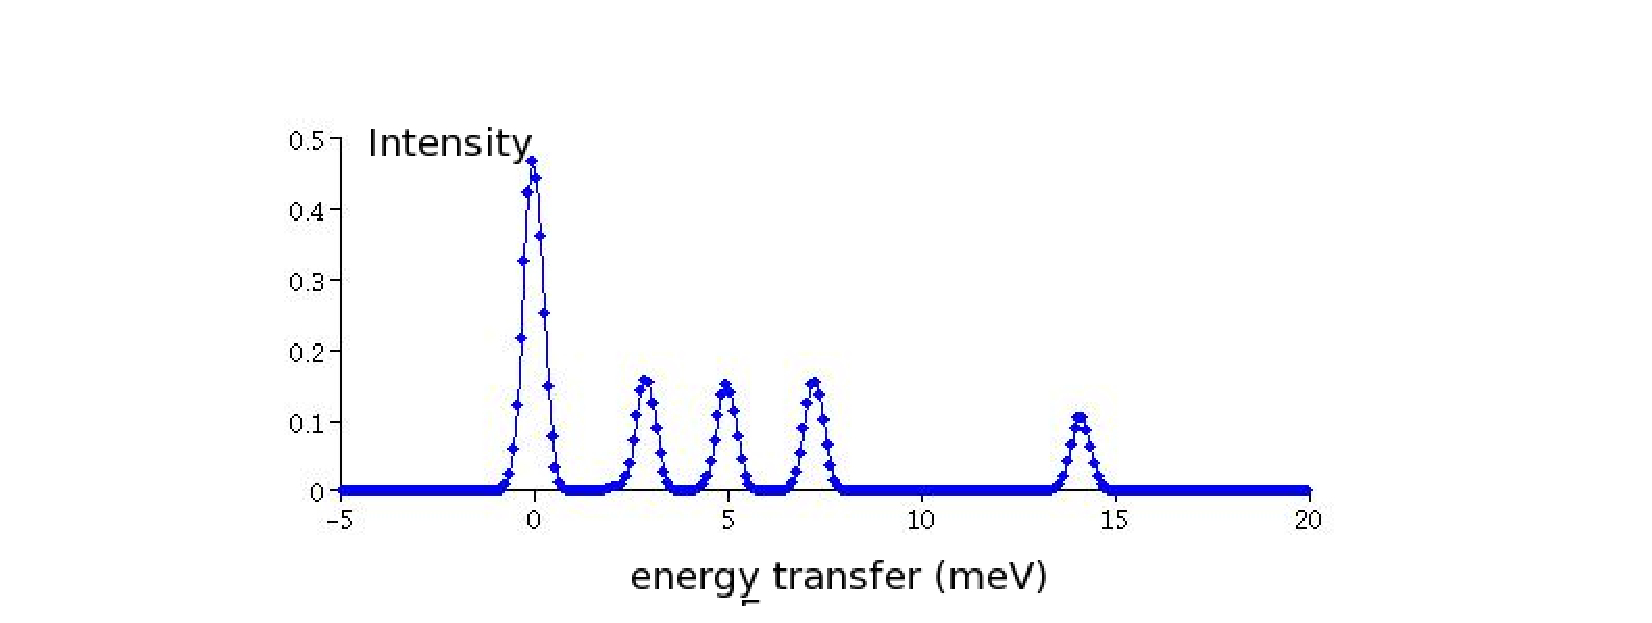
\includegraphics[angle=0,width=1.0\textwidth]{figsrc/10KCEFspectrum.eps}
\caption{\label{spectrum}
Calculated crystal field neutron spectrum of NdCu$_2$ at a temperature of 10~K.
Horizontal axis is energy transfer in meV and vertical axis is neutron intensity
in barns per meV and Nd atom and sr.
[plot created by program {\prg display}]}
\end{center}
\end{figure}
\item In order to calculate the magnetisation for our problem (in the paramagnetic state), 
 the magnetic field has to be given in the command line and
program {\prg singleion\index{singleion}} has to be started with the option {\prg -M}, i.e. 

{\bf so1ion -M -r Nd3p.sipf 10 0 0 1 0 0 0}

 The
numbers denote a temperature (10~K) and  a field 1 Tesla along the z-axis.
 By default the results are written directly to the screen, however they can be piped into
a file by 

{\bf so1ion -M -r Nd3p.sipf 10 0 0 1 0 0 0 >> results/moment.rtplot}

Here the ''>>'' sign appends the ouput of each command, thus iterating the 
command for several different magnetic fields allows to calculate a 
magnetisation curve -  fig.~\ref{moment} shows the result.

\begin{figure}[ht]
\begin{center}
\includegraphics[angle=0,width=0.7\columnwidth]{figsrc/moment.eps}
\caption{\label{moment}
Calculated magnetic moment for field applied along $x$ direction ($c$ axis, note the
notation of the crystal field $xyz$ axes with respect to the crystal lattice is
$xyz||cab$ in our example)
 of NdCu$_2$ at a temperature of 10~K.
[plot created by program {\prg gnuplot}]}
\end{center}
\end{figure}

\item In a similar way the temperature dependence of the susceptibility can be calculated, actually
one calculates the magnetisation at variable temperature.

\item The crystal field contribution to the specific heat may be calculated 
from the output file {\prg results/Nd3p.sipf.levels.cf} using the  program {\prg cpsingleion}\index{cpsingleion},
e.g. 

{\bf cpsingleion 10 100 1 results/Nd3p.sipf.levels.cef}
calculates the specific heat in the temperature interval 10-100 K with a step width
of 1 K. Alternatively a comparison to experimental data can be made by
 {\bf cpsingleion  1 2 cpexp.dat results/Nd3p.sipf.levels.cef},
where the temperatures are given in column 1 and the experimental specific heat in column
2 of file {\prg cpexp.dat}. The calculated specific heat is compared to the experimental data
 and
a standard deviation {\em sta} is calculated and output is written to stdout.
Other quantities can be calculated using the options: -s  (calculate entropy  (J/molK) instead of cp),
-f (calculate free energy (J/mol) instead of cp),-u  (calculate magnetic energy (J/mol) instead of cp),
-z (calculate partition sum instead of cp).
Fig.~\ref{cpndcu2} shows an example.
\begin{figure}[ht]
\begin{center}
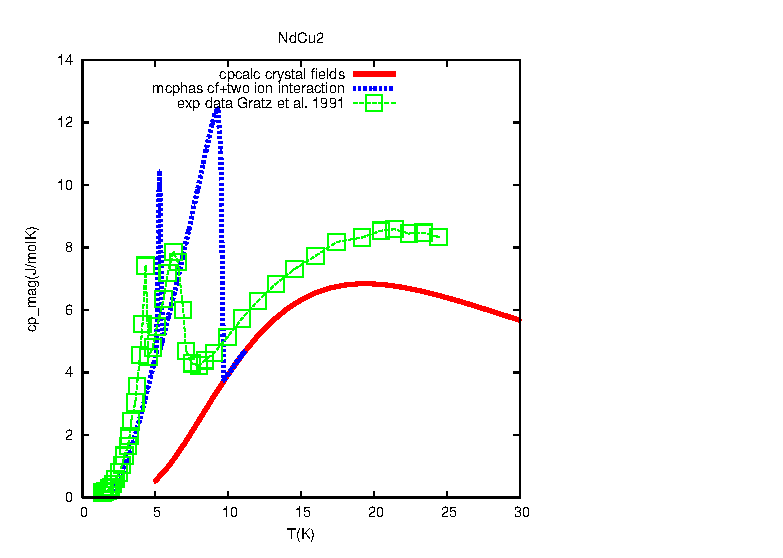
\includegraphics[angle=0,width=0.7\columnwidth]{figsrc/cpall.eps}
\caption{\label{cpndcu2}
Calculated specific heat of NdCu$_2$ in zero magnetic field as calculated
by {\prg cpsingleion} (crystal field contribution) in comparison with experimental
data~\cite{gratz91-9297}. The dashed line shows the results of a calculation,
which in addition to the crystal field takes into account the two ion interaction
and using {\prg singleion\index{singleion}} as a module in {\prg mcphas} - see below and chapter~\ref{runmcphas}.
[plot created by program {\prg gnuplot}]}
\end{center}
\end{figure}

\item The spin-disorder resistivity due to scattering of conduction $s$-electrons with the localised
$f$-electrons via the exchange interaction can be calculated in the first Born approximation as~\cite{raowallace},

\begin{equation} \label{eq:cfres}
\rho_{s-f}(T) = \frac{3\pi N m}{\hbar e^2 E_F} G^2(g-1)^2 \sum_{m_s,m_s',i,i'} 
      \langle m_s',i' | {\mathbf s \cdot J} | m_s, i \rangle^2 p_i f_{ii'}
\end{equation}

\noindent where $G$ is the exchange constant, $p_i$ is the Bose factor $e^{-\beta E_i}/Z$ and $f_{ii'}$ is the
Fermi function $2/(1+e^{-\beta(E_i-E_{i'})})$. The program {\prg rhoso1ion} can be used to calculate this
resistivity for magnetic ions in a crystal field. The wavefunctions $|i\rangle$ are taken from the file {\prg
results/Nd3p.sipf.levels.cef} output by {\prg singleion}. The matrix elements of ${\mathbf s \cdot J}$ are calculated according to
the formulae of Dekker~\cite{dekker}. {\prg rhoso1ion} calculates only the sum in the above equation, however.
The constant coefficient $\rho_0=(3\pi N m/\hbar e^2 E_F) G^2(g-1)^2$ is set to unity, or may be specified using
the option {\prg --rho0} or {\prg -r}. The syntax is otherwise the same as {\prg cpsingleion}. For example, to
calculate the resistivity from 10 to 100 K in 1 K steps with $\rho_0 = 0.2$~$\Omega$.cm, the command 

{\bf rhoso1ion 10 100 1 -r 0.2 -i results/Nd3p.sipf.levels.cef}

 can be used. Alternatively, for comparison with data,

 {\bf rhoso1ion 1 2 rhoexp.dat -r 0.2 -i results/Nd3p.sipf.levels.cef} 

can be used. Note that as the temperature dependence of the resistivity in this case is mainly a
function of the Bose and Fermi functions, at high temperatures where all $2J+1$ crystal field levels are
thermally occupied, the resistivity will saturate to a value $\rho_0 J(J+1)$.

\end{enumerate}

\vspace{1cm}
{\em Exercises:}
\begin{itemize}
\item Use {\prg singleion\index{singleion}} to calculate the energies, eigenvectors and
transition matrix elements (for inelastic
neutron scattering) for Nd$^{3+}$ in an orthorhombic crystal field.
Use the parameters given in section~\ref{cf1ion}.
\end{itemize}



\subsection{Using {\prg so1ion\index{so1ion}} as a module in {\prg McPhase} and {\prg McDisp}}
\label{cf1ion}


The use 
 of {\prg so1ion\index{so1ion}} as a module in {\prg mcphas} is necessary in order to 
 go beyond the capabilities of {\prg so1ion\index{so1ion}} (for instance the calculation
 of magnetisation or specific heat or if the exchange interaction
 given in equations~(\ref{hamilton}) and (\ref{multipolehamilton})
  shall be taken into account).  

\subsubsection{Module Tasks:}


As a single ion module, {\prg so1ion\index{so1ion}} provides to {\prg mcphas} the magnetic properties
of a single rare earth ion subject to the crystal field. Its main duty is
to calculate the magnetic moment given an effective magnetic field. 
To be more explicit - given the effective magnetic field $H^s_{eff}$ by {\prg mcphas}
 the module {\prg so1ion\index{so1ion}}
 diagonalises the crystal field and Zeeman Hamiltonian (\ref{cfze}) of the
 ion $n$:

\begin{equation}\label{cfze}
 {\mathcal H_n}=  B_l^m O_{lm}({\mbf J}^n) 
	     -  g_{Jn} \mu_B {\mbf J}^n {\mbf H^n_{eff}} 
\end{equation}

and calculates the expectation value of the angular momentum
 $\langle \mbf J^n \rangle$
according to

\begin{equation}
\langle \mbf J^n \rangle =
\sum_{\Gamma} p_{\Gamma} \langle \Gamma | \mbf J^n | \Gamma \rangle
\end{equation}

with 

\begin{eqnarray}
p_{\Gamma}&=&\frac{\exp(-E_{\Gamma}/kT)}{z}\\
z&=&\sum_{\Gamma} \exp(-E_{\Gamma}/kT)
\end{eqnarray}

Here $z$ is the partition sum, $|\Gamma\rangle$ the eigenstate corresponding to
the eigenvalue $E_{\Gamma}$ of the Hamiltonian (\ref{cfze}). 
\footnote{In addition to $\langle \mbf J_i \rangle$ the module also returns
the partition sum $z$ and the magnetic energy $u=\sum_{\Gamma} p_{\Gamma} E_{\Gamma}$.}

\subsubsection{Module Usage:}
 

The program {\prg mcphas} (-calculation of the magnetic phase diagram) 
requires a single ion
property input file of the same format as given above in
section~\ref{cfieldexample} (also for each ion in the
crystallographic unit cell):

\begin{itemize}
\item The first line in the single ion property file tells {\prg mcphas} that the module
{\prg so1ion\index{so1ion}} should be used for this ion. 
\item Comment lines start with \#. 
\item The type of ion has to be given plus
several lines containing the crystal field parameters. 
\end{itemize}

It follows a simple  example (for more complicated examples see section \ref{sifile} and 
{\prg mcphas.cf1} in the 
directory {\prg examples/ndcu2b\_new}):


\begin{verbatim}
#!MODULE=so1ion
#<!--mcphas.cf-->
# comment followed by
# the ion type and the crystal field parameters [meV]
 IONTYPE=Nd3+
# - note you can also do any pure spin problem by entering e.g. IONTYPE=S=2.5 
 B20=  0.116765                                           
 B22  =  0.134172                                           
 B40  =  0.0019225                                          
 B42  =  0.0008704                                          
 B44  =  0.0016916                                          
 B60  =  0.0000476                                          
 B62  =  0.0000116                                          
 B64  =  0.0000421                                          
 B66  =  0.0003662                                          
\end{verbatim}


\begin{description}
\item [Note:] 
In order to use {\prg so1ion\index{so1ion}} as a module in {\prg McPhase} a convention for
the orientation of the $xyz$ coordinate system (of the crystal field) relative
to the crystal axis $abc$ has to be made:
 The axes convention adopted in module {\prg so1ion} for the crystal field parameters
is - $\vec a||x$, $\vec b||y$ and $\vec c||z$. \footnote{Note that if you use the
module {\prg cfield}, the choice is more unconventional:$\vec a||y$, $\vec b||z$ and $\vec c||x$
Tools for rotating crystal field parameters are described in appendix~\ref{rotateBlm}.}
In case of non-orthogonal axes the convention 
is $y||\vec b$, $z||(\vec a \times \vec b)$ and $x$ perpendicular to $y$ and $z$.


The reason for
this unique choice is to make it possible to treat quadrupolar interactions - the 
generalisation of bilinear interactions to these higher order interactions
is much easier in a unique axes convention.



{\small
{\bf Information for experienced users:} the first line in the single ion property file
can either refer to  one of the standard
single ion property modules (e.g. Kramers ground state
doublet \#!MODULE=kramers, full crystal field \#!MODULE=so1ion) or a shared library file, which will be %%@
loaded
dynamically into the program at runtime 
 - for a description
of this file see section~\ref{sifile}.
}
